\documentclass{article}
\usepackage[utf8]{inputenc}
\usepackage{graphicx}
\usepackage{caption}
\usepackage{indentfirst}
\usepackage{float}
\usepackage[left=3cm,right=3cm,top=3cm,bottom=3cm]{geometry} 
\graphicspath{ {images/} }


\title{Creating different Web servers and a Web Benchmark tool}
\author{
Academic Area of Computer Engineering\\
CE-4303 – Operating Systems Principles\\
Rony Paniagua Chacón\\
Bryan Abarca Weber\\
Raúl Arias Quesada}
\date{April 2019}

\begin{document}

\maketitle

\section{Introduction}
A container is a standard unit of software that packages up code and all its dependencies so the application runs quickly and reliably from one computing environment to another. A Docker container image is a lightweight, standalone, executable package of software that includes everything needed to run an application: code, runtime, system tools, system libraries and settings \cite{WhatDocker}.\\
Docker Engine creates simple tooling and a universal packaging approach that bundles up all application dependencies inside a container. Docker Engine enables containerized applications to run anywhere consistently on any infrastructure, solving “dependency hell” for developers and operations teams, and eliminating the “it works on my laptop!” problem \cite{DockerEngine}.
\\For the implementation of the web server fork, it is necessary to use the system call fork, this system call is responsible for creating a "child" process, therefore the instructions after the fork will be executed in two processes.
\\This works by creating a clone of the process that executes the fork (parent process). The child process and the parent process run in separate memory spaces. At the time of fork () both memory spaces have the same content, but the changes made by each one are not reflected in the other.
\\Each of the processes has a unique process id, at the moment of executing the fork it returns:
\begin{enumerate}
    \item A negative value if the creation of a child process was unsuccessful.
    \item Zero to the newly created child process.
    \item A positive value, the process ID of the child process, to the parent.\cite{Fork}.
\end{enumerate}
In the case of the web server uses this system call to create a new child process, every time a new request arrives at the web server, the child process will be responsible for responding to the request, while the parent process will keep listening and accepting new requests.
\\The implementation of this is shown in the figure \ref{fig:intFork}, where after performing the fork it is queried by the zero value returned by the fork to identify the child process and this process is dedicated to answering the request.
\begin{figure}[H]
	\centering
	\captionsetup{justification=centering, margin=1cm}
    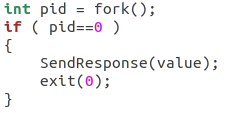
\includegraphics[width = 0.3\textwidth]{intFork.png}
    \caption{Fork usage in web server.}
	\label{fig:intFork}
\end{figure}
For the implementation of the web server thread, it is necessary to use the threads in C these can be used through the pthread library. 
\\A thread is defined as a sequence of such instructions within a program that can be executed independently of another code. The threads show some differences with the processes as they are:
\begin{enumerate}
    \item The process identifier is unique within the system, while the thread identifier is unique within the process.
    \item The processes use different memory spaces while the threads are within the same process address space, thus, much of the information presented in the memory description of the process can be shared across threads. Some information can not be replicated, such as the stack (stack pointer to a different memory area per thread), registers and thread-specific data. This information sufficient to allow threads to be scheduled independently of the program's main thread and possibly one or more other threads within the program.
\end{enumerate}
In the case of the web server use threads every time a new request arrives at the web server, the new thread will be responsible for responding to the request, to create the thread we use the function pthread\_create which receives the following parameters :
\begin{enumerate}
    \item The first argument is a pthread\_t type address. Once the function is called successfully, the variable whose address is passed as first argument will hold the thread ID of the newly created thread.
    \item The second argument may contain certain attributes like priority.
    \item The third argument is a function pointer, which is the function that the thread will execute.
    \item The fourth argument is the arguments that the function to execute receives, which can pass these arguments in form of a pointer to a void type.\cite{Thread}.
\end{enumerate}
The function returns zero in case of successful thread creation but returns the error number
\\The figure \ref{fig:intThread} shows the way the threads are created.
\begin{figure}[H]
	\centering
	\captionsetup{justification=centering, margin=1cm}
    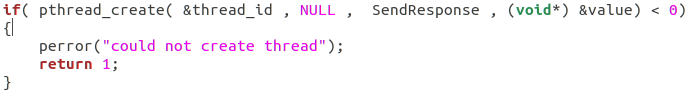
\includegraphics[width = \columnwidth]{intThread.png}
    \caption{Thread usage in web server}
	\label{fig:intThread}
\end{figure}

When there are processes, threads in this case, that need to use the same resource of the computer to execute their functions, the system in charge of administering such resource, should look for a solution to allow all the threads to complete their execution. This problem gives rise to algorithms capable of deciding which process is allowed to run and coordinate the use of resources among all other processes. Therefore, to manage the threads used in the threaded server, scheduling algorithms are used, based on the Selfish Round Robin, Lottery and Real Time type schedulers.\\
The objective of the Selfish Round Robin is to give better service to processes that have been executing for a while than to newcomers. Its a more logical and superior implementation compared to the normal Round Robin algorithm \cite{SRR}. Its functionality is as follows:
\begin{itemize}
    \item Processes in the ready list are partitioned into two lists: NEW and ACCEPTED.
    \item The New processes wait while Accepted processes are serviced by the Round Robin.
    \item Priority of a new process increases at rate ‘a’ while the priority of an accepted process increases at rate ‘b’.
    \item When the priority of a new process reaches the priority of an accepted process, that new process becomes accepted.
    \item If all accepted processes finish, the highest priority new process is accepted.
\end{itemize}
Lottery Scheduling is type of process scheduling, somewhat different from other Scheduling. Processes are scheduled in a random manner. Lottery scheduling can be preemptive or non-preemptive. It also solves the problem of starvation. Giving each process at least one lottery ticket guarantees that it has non-zero probability of being selected at each scheduling operation \cite{Lottery}. In this scheduling every process have some tickets and scheduler picks a random ticket and process having that ticket is the winner and it is executed for a time slice and then another ticket is picked by the scheduler. A process having a higher number of tickets give it more chance to get chosen for execution \cite{Lottery}.\\
The implemented real-time planning algorithm uses two queues, one for real-time processes and one for other processes in general. These two queues implement a Round Robin scheduling algorithm but as long as there are processes in the real-time queue, no process of the general process queue is attended.

\section{Development environment}
For the development of this project the tools were necessary:
\begin{enumerate}
    \item Operating system with Linux distribution preferably Ubuntu.
    \item C code editor, you can even use the text editor of the operating system, in our case we use the free editor Visual Studio Code.
    \item Dockers: open source project used for the creation and testing of dockers, which use:
    \begin{itemize}
        \item Docker Container: they are used to implement the services, each Docker contains the resources and necessary configuration of the environment that each of the services needs for its operation. Dockers bundle up all application dependencies inside container and enables containerized applications to run anywhere on any infrastructure \cite{DockerEngine}.\\
        In other words, with Docker, it is possible to grab a portable runtime environment as an image, no installation necessary. Then, the build can include the base environment image right alongside your app code, ensuring that your app, its dependencies, and the runtime, all travel together \cite{DockerContainer}.
        These portable images are defined by something called a Dockerfile \cite{DockerContainer}.
        \item Dockerfile: defines what goes on in the environment inside your container. Access to resources like networking interfaces and disk drives is virtualized inside this environment, which is isolated from the rest of your system, so you need to map ports to the outside world, and be specific about what files you want to “copy in” to that environment. However, after doing that, you can expect that the build of your app defined in this Dockerfile behaves exactly the same wherever it runs \cite{DockerContainer}.
    \end{itemize}
\end{enumerate}

\section{Details of program design}
\subsection{Web server FIFO}
To install Docker Community Edition and its dependencies an automation script was created. In this script also is built and runned a docker, using the Dockerfile in the current directory, the content of this file is explained later.

\begin{figure}[H]
	\centering
	\captionsetup{justification=centering, margin=1cm}
    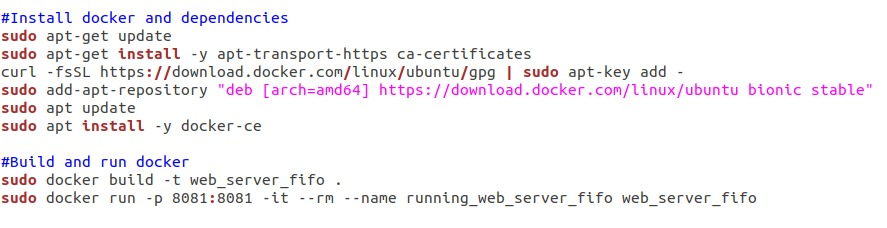
\includegraphics[width = 0.01\textwidth]{installdocker.jpeg}
    \caption{Docker installer script.}
	\label{fig:installdocker}
\end{figure}

In contrast, to stop the docker container execution and uninstall it, the following script is executed.

\begin{figure}[H]
	\centering
	\captionsetup{justification=centering, margin=1cm}
    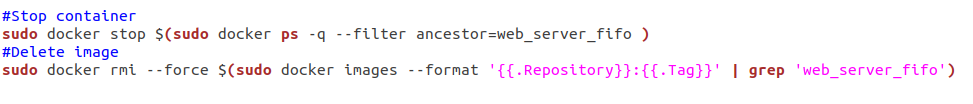
\includegraphics[width = \columnwidth]{removedocker.png}
    \caption{Docker uninstaller script.}
	\label{fig:removedocker}
\end{figure}

To create a daemon service within the docker it is necessary to create a script that contains the operations of starting, stopping, restarting and viewing the state of the daemon, which has the content shown in the following figure.

\begin{figure}[H]
	\centering
	\captionsetup{justification=centering, margin=1cm}
    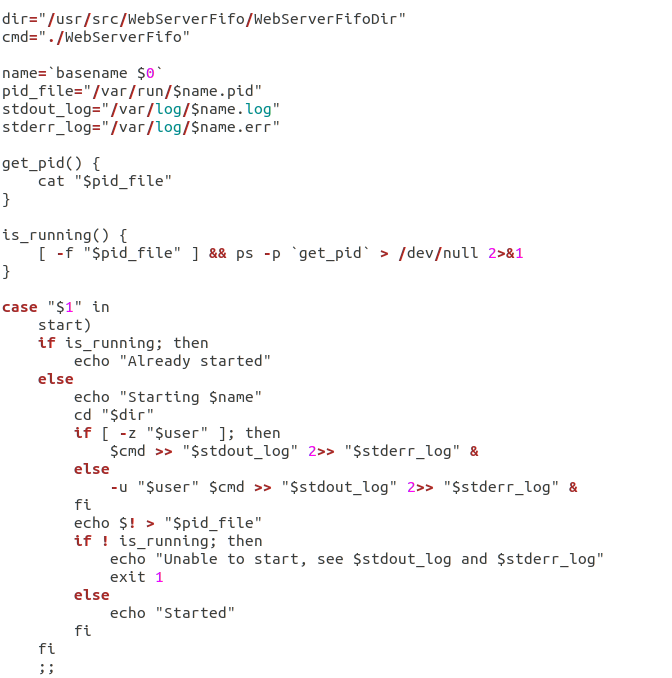
\includegraphics[width = \columnwidth]{installweb1.png}
    \caption{Web Server service installer script.}
	\label{fig:installweb1}
\end{figure}
\begin{figure}[H]
	\centering
	\captionsetup{justification=centering, margin=1cm}
    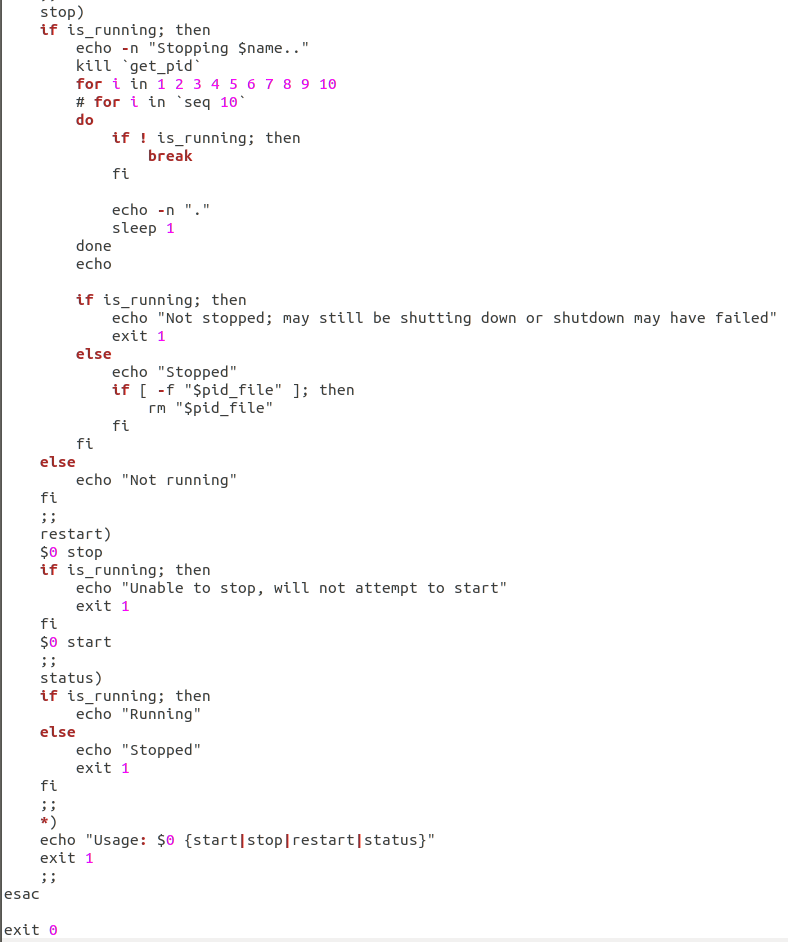
\includegraphics[width = \columnwidth]{installweb2.png}
    \caption{Web Server service installer script.}
	\label{fig:installweb2}
\end{figure}

The following script is used to stop and remove the web server daemon service. 

\begin{figure}[H]
	\centering
	\captionsetup{justification=centering, margin=1cm}
    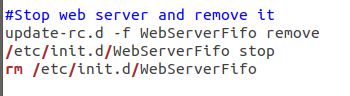
\includegraphics[width = 0.5\textwidth]{stopweb.png}
    \caption{Script to stop the web server daemon.}
	\label{fig:stopweb}
\end{figure}

As mentioned, what goes on in the environment inside a container is defined by a Dockerfile. For instance in this project the Dockerfile in the figure \ref{fig:docker}, were used.

\begin{figure}[H]
	\centering
	\captionsetup{justification=centering, margin=1cm}
    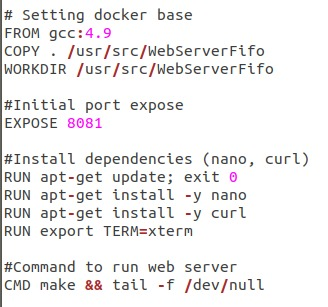
\includegraphics[width = 0.5\textwidth]{docker.jpeg}
    \caption{Dockerfile.}
	\label{fig:docker}
\end{figure}

In this file the environment inside the container is configured. First a gcc runtime environment is defined as the parent image, since the server application was implemented in C. The current directory contents are copied into the container at /usr/src/WebServerFifo, as well the working directory is set to the same directory.\\
The port 8081 is initially set available to the world outside this container. Then, all packages and dependencies needed are installed, and finally the Makefile is executed to perform the installation and configuration of the server when the container launches.\\
The Makefile content is presented in the figure \ref{fig:makefile}.

\begin{figure}[H]
	\centering
	\captionsetup{justification=centering, margin=1cm}
    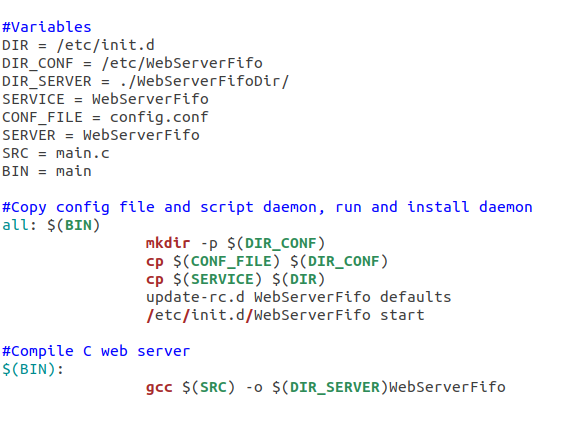
\includegraphics[width = 0.7\textwidth]{makefile.png}
    \caption{Makefile to install and configure the server.}
	\label{fig:makefile}
\end{figure}

The instructions in the Makefile are executed inside the docker container to install the web server. First the source code of this web server is compiled, generating a binary file located in /WebServerFifoDir in the current directory. Next the config file and the daemon script are copied to their respective folders and finally the daemon is installed and runned.\\

The web server has a main.c file that contains the functionality of it, based on \cite{Server}.
With the following methods:
\begin{enumerate}
    \item startServer: this method receives the port as input, it is responsible for lifting the web server, executing the socket and bind actions of the server, this using the sys / socket.h library.
    \item SendResponse: It receives as input the request to answer, it is responsible for verifying the request and responding using HTTP-1.1 for it, it executes methods such as recv to read the request and write to respond.
    \item main: Main method responsible for reading the values of configuration files, raise the server and keep listening and accepting connections using the other methods created.
    \item getLogPath: Method that reads the configuration file and returns the path for the file where to write the logs, for it looks for the line that has the value of "LOGFILE", in case of not finding the value of the path it returns the value for defect /var/log/syslog. Use methods such as fopen to open the file, fgets to read lines from the file, and sscanf to find the correct line.
    \item getPort: Method that reads the configuration file and returns the port to use, for it looks for the line that has the value of "PORT", in case of not finding the value of the port it returns the default value 8081. It uses methods as fopen to open the file, fgets to read lines from the file and sscanf to find the correct line.
    \item write: Receive the data to write and the path of the file to write, in addition to writing the required message write the time of the system to have a better log of the activity. Use the time.h library to get the time and methods such as open to open the file and write to write to it.
\end{enumerate}
\subsection{Web server Fork}
Below are the main differences that the web server fork has, most of the files maintain their structure (docker, makefile, installation scripts and uninstallation).
\\The web server has a main.c file that contains the functionality of it, based on \cite{Server}, which contains the following differences:
\begin{itemize}
    \item Use of the fork method to handle client requests.
    \item Some global attributes now are method attributes due to the multi processes.
\end{itemize}
\subsection{Web server Thread}
Below are the main differences that the web server thread has, most of the files maintain their structure (docker, makefile, installation scripts and uninstallation).
The web server has a main.c file that contains the functionality of it, based on \cite{Server}, which contains the following differences:
\begin{itemize}
    \item Each time a request arrives, a thread is created that responds to the request.
    \item Some global attributes now are method attributes due to the multi threads. 
    \item in the config file the SCHEDULER parameter is added, which indicates the type of scheduler to be used. The default scheduler is the selfish round robin, the possible values of this parameter are: SRR for Selfish Round Robin, RT for Real Time and LOT for Lottery
\end{itemize}

\subsection{Round Robin Scheduler}
This algorithm works in the following way.
The following figure presents the section of the code that is responsible for distributing the execution times to the processes and making the context changes. 
\begin{figure}[H]
	\centering
	\captionsetup{justification=centering, margin=1cm}
    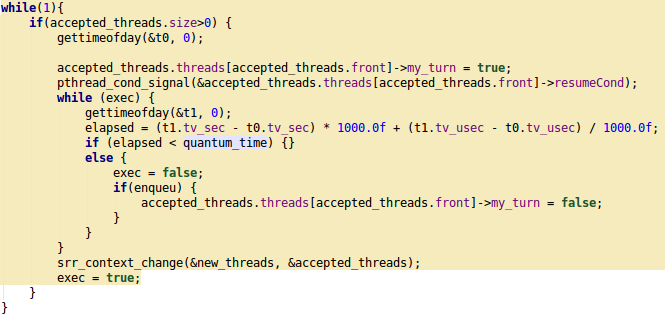
\includegraphics[width = 0.7\textwidth]{SRR.png}
    \caption{Code section of SRR scheduler algorithm.}
	\label{fig:SRR}
\end{figure}
Each process has an attribute called my\_turn which indicates when a process should be executed or paused. To put the threads or processes in pause the pthread\_cond\_wait method is used, and to put these back on, pthread\_cond\_signal is used.
By default, each quantum is composed of 2 ticks of 50 milliseconds, but the user can specify it in the configuration file.\\
When the execution time of a process finishes, the srr\_context\_change function is called to perform a context change.
Roughly, this method is responsible for adding the priority corresponding to each process of the two queues, the ACCEPTED and NEW queues. \\
Then check if there are processes in the NEW queue, with priority greater than or equal to that of the process with the lowest priority in the ACCEPTED queue. If so, send these processes to the ACCEPTED queue. \\
For the management of these processes, a structure was constructed that contains the attributes of each process. These structures are stored in an array.\\
The following figure shows the attributes that are stored in each process.
\begin{figure}[H]
	\centering
	\captionsetup{justification=centering, margin=1cm}
    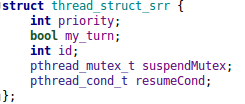
\includegraphics[width = 0.7\textwidth]{structSRR.png}
    \caption{Structure uses by the SRR scheduler algorithm.}
	\label{fig:structSRR}
\end{figure}
The priority attribute indicates the priority of the process, my\_turn has already been explained above, it indicates whether the process should be paused or running, the id is an identifier for easier handling of the processes, and the last two attributes allow to put the thread in pause or running.

\subsection{Lottery Scheduler}
Like the previous scheduler, the lottery scheduler has the following piece of code that controls the order and execution time of the processes.
\begin{figure}[H]
	\centering
	\captionsetup{justification=centering, margin=1cm}
    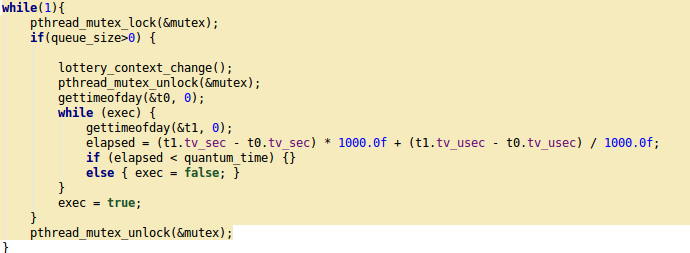
\includegraphics[width = 0.7\textwidth]{lottery.png}
    \caption{Code section of lottery scheduler algorithm.}
	\label{fig:lottery}
\end{figure}
This scheduler algorithm is simpler than the past, since it only calls the lottery\_context\_change method that is in charge of making the raffle among the tickets of all the processes, and the winner obtains the following execution time.\\
For the management of these processes, a structure was constructed that contains the attributes of each process. These structures are stored in an array. The following figure shows the attributes that are stored in each process.
\begin{figure}[H]
	\centering
	\captionsetup{justification=centering, margin=1cm}
    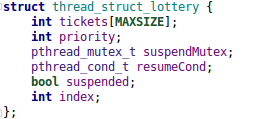
\includegraphics[width = 0.7\textwidth]{structLottery.png}
    \caption{Structure uses by the lottery scheduler algorithm.}
	\label{fig:structLottery}
\end{figure}
In the tickets attribute the tickets that the scheduler assigns to the process are stored, the variable priority indicates the priority of the process or rather the amount of tickets that are given, the suspended attribute indicates if the process should be executed or paused, the index attribute is an identifier to facilitate the handling of structures, pthread\_mutex\_t and pthread\_cond\_t are used to put the thread on pause or execution. 
\subsection{Real-time Scheduler}
\begin{figure}[H]
	\centering
	\captionsetup{justification=centering, margin=1cm}
    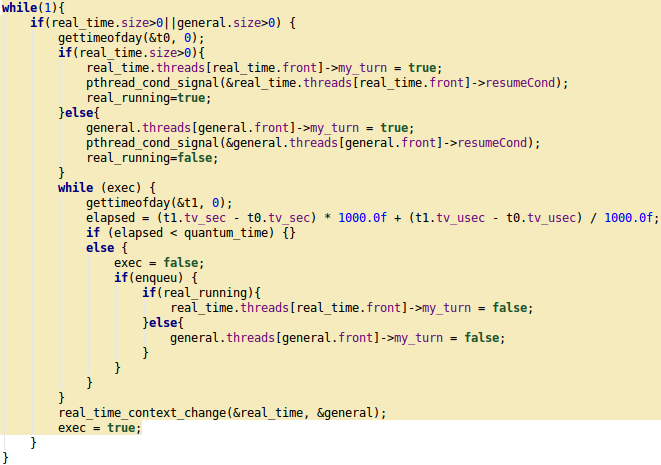
\includegraphics[width = 0.7\textwidth]{realtime.png}
    \caption{Code section of real-time scheduler algorithm.}
	\label{fig:realtime}
\end{figure}
This code corresponds to that of the real-time scheduler, this algorithm manages the execution times of the processes in the following way:
There are two process queues, one for real time processes and one for other processes. When there is at least one real-time process, such as a video for example, in the queue of real-time processes, this or these are executed until there are no more waiting in this queue, when there are no longer real-time processes, the processes from the other queue are attended.
\begin{figure}[H]
	\centering
	\captionsetup{justification=centering, margin=1cm}
    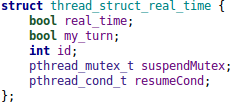
\includegraphics[width = 0.7\textwidth]{structRealtime.png}
    \caption{Structure uses by the real-time scheduler algorithm.}
	\label{fig:structRealtime}
\end{figure}
This is the structure created to handle the processes in this scheduler. The variable real\_time indicates if the process is real time or not, the attribute my\_turn is used to indicate when the process must be executed or paused, id is used to identify the process and the last two attributes allow to put the thread in pause or running.


\subsection{Benchmark tool}
The benchmark tool to develop is an application that will take the console parameters ($<$machine$>$ $<$port$>$ $<$file$>$r $<$N-threads$>$ $<$N-cycles$>$) and interpret them to create N number of threads with the mylpthread library where each one of these threads will open a connection socket to the server of the specified machine, each of these sockets will make the corresponding request the specified number of times. A general diagram is presented in the figure \ref{fig:BenchMarkDiagram} of how the benchmark tool works.\\
\begin{figure}[H]
	\centering
	\captionsetup{justification=centering, margin=1cm}
    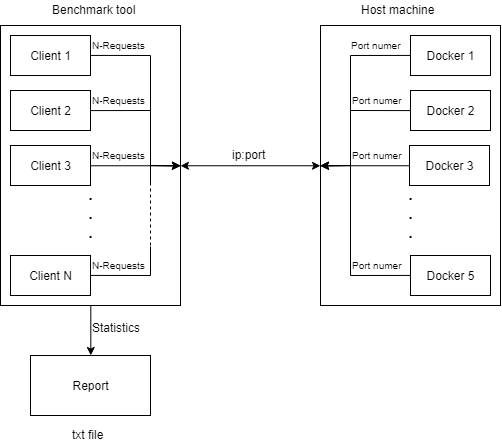
\includegraphics[width=\columnwidth]{BenchMarkDiagram.png}
    \caption{Benchmarck diagram.}
	\label{fig:BenchMarkDiagram}
\end{figure}
Each thread created for the requests will be in charge of storing the information of the corresponding times, that is, the average response time of the server in each request of the N cycles carried out. The time at which each of the cycles began to run will also be saved.\\
At the end of the test, general statistics of the result will be saved, such as: the date on which it was performed, the IP address and port of the server, the number of requests made, the type of file that was requested, the size of the file, the total seconds that the test took and the average response time of all requests made. Figure \ref{fig:benchReportExamp} shows an example of the format that the test report will have.\\
In the /program/benchmark-tool directory of the project an executable file is provided to be used from the terminal with the previously described parameters. Thus, in the same directory, the source file of the program is provided, which contains the following methods:
\begin{itemize}
    \item main: method which is executed by default. This is responsible for obtaining the parameters entered in the console for the execution of the tests, some of these are globally defined to be used by the socketConnection method. Creates the number of threads specified by the user and writes in the BenchMarkReport.csv file the general statistics obtained from the test.  This method waits until all the threads finish executing to finish the execution of the program.
    \item socketConnection: this method is the one that is executed by the threads. It is responsible for creating a socket with the specified ip and port, then creates a connection to this socket, which refers to the Docker where the server to which wanted to perform the queries, is located. Once the connection is established, it sends a HTTP / 1.0 GET request requesting the required file. During the reading of bytes sent by the server, it takes the time that this procedure takes. This process is performed the number of cycles indicated, then the average time of each query is obtained and written in the file BenchMarkReport.csv.
\end{itemize}

\begin{figure}[H]
	\centering
	\captionsetup{justification=centering, margin=1cm}
    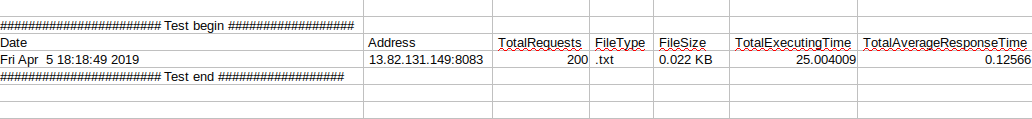
\includegraphics[width=\columnwidth]{benchmarkReportExamp.png}
    \caption{Benchmarck report example.}
	\label{fig:benchReportExamp}
\end{figure}

\section{Instructions of how to use the programs}

\subsection{Installation and use of the servers}
\subsubsection{Requirements}
\begin{itemize}
    \item Work with Ubuntu (tested on a azure VM with Ubuntu 18.04).
\end{itemize}

\subsubsection{Creation and execution of the docker}
To create the docker it is only necessary to execute the following commands, in the path where the delivered files are located, this is responsible for installing docker in the machine, do the docker build and execute it. It is necessary to add nano and curl to the docker, for that reason the installation commands are added to the docker, but when executing them some messages in red of some things that are not found are shown, however, this does not interfere in the correct functioning of the docker.\\
\newline
\centerline{Fifo web server: sh InstallDockerFifo.sh}
\centerline{Fork web server: sh InstallDockerFork.sh}
\centerline{Thread web server: sh InstallDockerThread.sh}


\subsubsection{Docker execution test}
When executing the previous command, the docker remains running. By default it is ready to run on port 8081 (Fifo web server), 8083 (Fork web server), 8085 (Thread web server) so to do tests it would only be necessary to go to a browser and make requests. Currently there are several test files in the directory of the web server:\\
\newline
\centerline{Fifo web server: (/usr/src/WebServerFifo/WebServerFifoDir)}
\centerline{Fork web server: (/usr/src/WebServerFork/WebServerForkDir)}
\centerline{Thread web server: (/usr/src/WebServerThread/WebServerThreadDir)}
\newline
\\So the possible requests would be:\\
\newline
\centerline{http://server:port/test.png}
\centerline{http://server:port/test.pdf}
\centerline{http://server:port/test.html}
\centerline{http://server:port/test.bin}
\centerline{http://server:port/test.mp4}
		
\subsubsection{Modify web server config and operations with the daemon}
To enter the running docker you must open another terminal and execute the command:\\ 
\newline
\centerline{Fifo web server: sudo docker exec -it running\_web\_server\_fifo bash}	
\centerline{Fork web server: sudo docker exec -it running\_web\_server\_fork bash}
\centerline{Thread web server: sudo docker exec -it running\_web\_server\_thread bash}
\newline\\
To perform the requested operations (start, stop, restart, view status) of the web server, as well as modify the configuration file, the following commands must be executed:\\
\newline
To perform actions on the daemon Fifo\\
\newline
\centerline{Start daemon: /etc/init.d/WebServerFifo start}
\centerline{Stop daemon: /etc/init.d/WebServerFifo stop}
\centerline{Restart daemon: /etc/init.d/WebServerFifo restart}
\centerline{Daemon status: /etc/init.d/WebServerFifo status}
\newline\\
To perform actions on the daemon Fork\\
\newline
\centerline{Start daemon: /etc/init.d/WebServerFork start}
\centerline{Stop daemon: /etc/init.d/WebServerFork stop}
\centerline{Restart daemon: /etc/init.d/WebServerFork restart}
\centerline{Daemon status: /etc/init.d/WebServerFork status}
\newline\\
To perform actions on the daemon Thread\\
\newline
\centerline{Start daemon: /etc/init.d/WebServerThread start}
\centerline{Stop daemon: /etc/init.d/WebServerThread stop}
\centerline{Restart daemon: /etc/init.d/WebServerThread restart}
\centerline{Daemon status: /etc/init.d/WebServerThread status}
\newline\\
To modify the configuration file\\
\newline
\centerline{Fifo web server: nano /etc/WebServerFifo/config.conf}
\centerline{Fork web server: nano /etc/WebServerFork/config.conf}
\centerline{Thread web server: nano /etc/WebServerThread/config.conf}

\subsubsection{Uninstall docker}
To uninstall the docker it is necessary to execute the command in the path where the delivered files are located:\\
\newline
\centerline{Fifo web server: sh RemoveDockerFifo.sh}
\centerline{Fork web server: sh RemoveDockerFork.sh}
\centerline{Thread web server: sh RemoveDockerThread.sh} 

\subsection{Use the benchmark-tool}
To use the benchmark-tool it is necessary to go to the /program/benchmark-tool directory within the project directories. Execute the Makefile with the command "make" (in the terminal) to create the executable file. Then the following command must be executed from the terminal to perform tests:\\
\centerline{./bclient $<$ip$>$ $<$port$>$ $<$file$>$ $<$N-threads$>$ $<$N-cycles$>$
}
Where:
\begin{itemize}
    \item ip: ip address of the Docker where the servers are running.
    \item port: port of the Docker where the specific server (FIFO, Fork, etc).
    \item file: the file the test will request for. Is necessary specify the extension of the file, for example: file.txt.
    \item N-threads: the quantity of threads the benchmark will create to generate requests at the same time.
    \item N-cycles: the quantity of requests each thread will send.
\end{itemize}
After running the test, a file called BenchMarkReport.csv will be created where the test results will be saved as shown in the figure \ref{fig:benchReportExamp}. If you have already done tests before, the new results will be saved in the same file without being overwritten, therefore, if you want to clean the test history you must delete them manually in the file, or delete it from the directory

\section{Student activity log}

\begin{table}[H]
\centering
\caption{Bryan Abarca Activity Log}
\begin{tabular}{|p{7cm}|p{7cm}|}
\hline
\textbf{Activity} & \textbf{Duration} \\ \hline
Reading and analysis of the project specification. & 1 h \\ \hline
Research on the operation and use of docker containers. & 2 h\\ \hline
Implementation of the docker container and and adjustments in the makefile. & 6 h\\ \hline
Documentation phase 1. & 3 h\\ \hline
Research on the thread server. & 2 h\\ \hline
Implementation of thread server. & 4 h\\ \hline
Create all scripts of thread server. & 2 h\\ \hline
Analysis and creation of pseudocode of selfish round robin scheduler. & 1 h\\ \hline
Analysis and creation of pseudocode of real time scheduler. & 1 h\\ \hline
Analysis and creation of pseudocode of lottery scheduler. & 1 h\\ \hline
Implementation lottery scheduler. & 3 h\\ \hline
Documentation phase 2. & 3 h\\ \hline
Total & 29 h\\ \hline
\end{tabular}
\end{table}

\begin{table}[H]
\centering
\caption{Raúl Arias Activity Log}
\begin{tabular}{|p{7cm}|p{7cm}|}
\hline
\textbf{Activity} & \textbf{Duration} \\ \hline
Reading and analysis of the project specification. & 1 h \\ \hline 
Error correction of FIFO web server (logs, makefile, uninstall file). & 4 h  \\ \hline
Research on the operation and use of docker containers. & 2 h \\ \hline
Support in the creation of the docker. & 2 h \\ \hline
Implementation of the daemon for SysV. & 2 h \\ \hline
Documentation phase 1. & 2 h\\ \hline
Research on the fork server. & 1 h\\ \hline
Implementation of fork server. & 3 h\\ \hline
Create all scripts of fork server. & 2 h\\ \hline
Analysis and creation of pseudocode of selfish round robin scheduler. & 1 h\\ \hline
Analysis and creation of pseudocode of real time scheduler. & 1 h\\ \hline
Analysis and creation of pseudocode of lottery scheduler. & 1 h\\ \hline
Implementation selfish round robin scheduler. & 4 h\\ \hline
Documentation phase 2. & 3 h\\ \hline
Total & 29 h \\ \hline
\end{tabular}
\end{table}

\begin{table}[H]
\centering
\caption{Rony Paniagua Activity Log}
\begin{tabular}{|p{7cm}|p{7cm}|}
\hline
\textbf{Activity} & \textbf{Duration} \\ \hline
Reading and analysis of the project specification. & 1 h \\ \hline
High level design of the benchmark. & 3 h\\ \hline
Research on the operation and use of docker containers. & 2 h\\ \hline
Implementation of the installation and destruction script of the docker container. & 2 h\\ \hline
Documentation phase 1. & 3 h\\ \hline
Research on the creation of benchmark. & 2 h\\ \hline
Implementation of benchmark & 5 h\\ \hline
Analysis and creation of pseudocode of selfish round robin scheduler. & 1 h\\ \hline
Analysis and creation of pseudocode of real time scheduler. & 1 h\\ \hline
Analysis and creation of pseudocode of lottery scheduler. & 1 h\\ \hline
Implementation real time scheduler. & 3 h\\ \hline
Documentation phase 2. & 3 h\\ \hline
Total & 27 h\\ \hline
\end{tabular}
\end{table}

\section{Project final status}
So far we have the successful implementation of the docker that contains the fifo web server, the docker that contains the fork web server and the docker that contains the thread web  which works correctly without errors detected.
\\At this point we have not been able to perform the own implementation of the pthread library.
\section{Conclusions}
The use of dockers presents a series of advantages such as the compatibility that allows to execute applications independently of the platform in which they are being executed, besides it allows to realize a standardization and simplicity of configurations, all the previous allows the deploy of applications to be much easier and faster regardless of the platform used.
\section{Suggestions}
It is recommended to start with images of dockers that have installed some of the components that are needed, for example the start of the docker from gcc avoids having to add the commands necessary for the installation of gcc
\section{References}
\begin{thebibliography}{1}

\bibitem{WhatDocker}
Docker. [Online]. Available: https://www.docker.com/resources/what-container

\bibitem{DockerEngine}
Docker. [Online]. Available: https://www.docker.com/products/docker-engine

\bibitem{DockerContainer}
docker docs. Get started, part 2: Containers. [Online]. Available: https://docs.docker.com/get-started/part2/

\bibitem{Server}
Rastogi, A. (2010). A Very Simple HTTP Server writen in C. [Online]
Abhijeet’s Blog. Available: https://blog.abhijeetr.com/2010/04/very-
simple-http-server-writen-in-c.html.

\bibitem{Fork}
fork(2) - Linux manual page, Man7.org. [Online]. Available:
\\http://man7.org/linux/man-pages/man2/fork.2.html.

\bibitem{Thread}
Multithreaded Programming (POSIX pthreads Tutorial), Randu.org. [Online]. Available: \\https://randu.org/tutorials/threads/. 

\bibitem{SRR}
Operating System | Selfish Round Robin Scheduling, Geeksforgeeks.org. [Online]. Available:https://www.geeksforgeeks.org/operating-system-selfish-round-robin-scheduling/

\bibitem{Lottery}
Operating System | Lottery Process Scheduling, Geeksforgeeks.org. [Online]. Available:https://www.geeksforgeeks.org/operating-system-lottery-scheduling/


\end{thebibliography}

\end{document}
